\section{Funktionen}
	\subsection{Aufgaben einer Funktion}
		\begin{compactitem}
			\item Gleichartige, funktional zusammengehörende Programmteile unter einem eigenen Namen zusammenfassen. Der Programmteil kann mit diesem Namen aufgerufen werden.
			\item Einige Funktionen (im speziellen mathematische) sollen parametrisiert werden können, z.B. die Cosinusfunktion macht nur Sinn, wenn sie mit unterschiedlichen Argumenten aufgerufen werden kann.
			\item Divide et impera (divide and conquer, teile und herrsche): Ein grosses Problem ist einfacher zu lösen, wenn es in mehrere einfachere Teilprobleme aufgeteilt wird.
		\end{compactitem}	
		
	\subsection{Definition von Funktionen \verweis{9.3.1}}
		\begin{minipage}[c]{10 cm}
			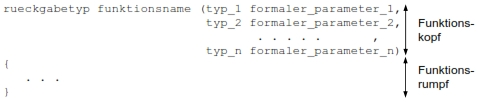
\includegraphics[width=1\textwidth]{pics/funktionen_aufbau.jpg}
		\end{minipage}
		%
		\begin{minipage}[c]{9 cm}
			\begin{compactitem}
				\item Funktionskopf: legt die Aufrufschnittstelle (Signatur) der Funktion fest. Er besteht aus Rückgabetyp, Funktionsname und Parameterliste.
				\item Funktionsrumpf: Lokale Vereinbarungen und Anweisungen innerhalb eines Blocks
			\end{compactitem}	
		\end{minipage}	
			
	\subsection{Eingaben/Ausgaben einer Funktion \verweis{9.3}}
		\begin{minipage}[t]{8.5 cm}
			\subsubsection{Eingabedaten}
				Es sind folgende Möglichkeiten vorhanden um Daten an Funktionen zu übergeben:
				\begin{compactitem}
					\item Mithilfe von Werten, welche an die Parameterliste übergeben werden
					\item Mithilfe von globalen Variablen
				\end{compactitem}
		\end{minipage}
		\hspace*{0.5cm}
		\begin{minipage}[t]{8.5 cm}
			\subsubsection{Ausgabedaten}
				Es sind folgende Möglichkeiten vorhanden um Daten zurückzugeben:
				\begin{compactitem}
					\item Mithilfe des Rückgabewertes einer Funktion ($return$)
					\item Mithilfe von Änderungen an Variablen, deren Adresse über die Parameterliste an die Funktion übergeben wurde
					\item Mithilfe von Änderungen an globalen Variablen
				\end{compactitem}	
		\end{minipage}	
		
		\subsubsection{Beispiele}
			\begin{minipage}[t]{8.5 cm}
				\textbf{Parameterlos und ohne Rückgabewert:}
				\lstinputlisting[language=C,tabsize=2]{code/funktionen_parameter_1.c}
				
				\textbf{Parameter und ohne Rückgabewert:}
				\lstinputlisting[language=C,tabsize=2]{code/funktionen_parameter_2.c}
			\end{minipage}
			\hspace*{0.5cm}
			\begin{minipage}[t]{8.5 cm}
				\textbf{Parameter und Rückgabewert:}
				\lstinputlisting[language=C,tabsize=2]{code/funktionen_parameter_3.c}
			\end{minipage}

	\subsection{Deklaration von Funktionen \verweis{9.4}}
		Es ist festgelegt, dass die Konsistenz zwischen Funktionskopf und Funktionsaufrufen vom Compiler überprüft werden soll. Dazu muss beim Aufruf der Funktion die Schnittstelle der Funktion, d.h. der Funktionskopf, bereits bekannt sein. Steht aber die Definition einer Funktion im Programmcode erst nach ihrem Aufruf, so muss eine Vorwärtsdeklaration der Funktion erfolgen, indem vor dem Aufruf die Schnittstelle der Funktion mit dem Funktionsprototypen deklariert wird. \\
		Desweitern ist zu beachten, dass Parameternamen im Funktionsprototyp und in der Funktionsdefinition nicht übereinstimmen müssen. Es ist jedoch zu empfehlen.
		
		\begin{minipage}[t]{9.5 cm}
			\subsubsection{Beispiel}
				\lstinputlisting[language=C,tabsize=2]{code/funktionen_prototyp.c}	
		\end{minipage}
		\hspace*{0.5cm}
		\begin{minipage}[t]{7.5 cm}	
			\subsubsection{Was passiert wenn der Prototyp vergessen geht?}
				\begin{compactitem}
					\item Fehlt der Prototyp ganz, so wird die Funktion implizit (automatisch vom System) deklariert. Ihr Rückgabetyp wird als $int$ angenommen, die Parameter werden nicht überprüft.
					\item Wenn die Funktion später definiert wird und nicht $int$ als Rückgabetyp hat, bringt der Compiler eine Fehlermeldung.
				\end{compactitem}
		\end{minipage}
		
		\subsubsection{Funktionsprototypen in der Praxis \verweis{9.4}}
			\begin{compactitem}
				\item Funktionsprototypen, welche die Schnittstelle der Unit beschreiben, kommen in das entsprechenden Headerfile.
				\item Jedes C-File, welches diese Schnittstelle nutzt, inkludiert dieses Headerfile und somit die Funktionsprototypen.
				\item Funktionsprototypen von internen Funktionen der Unit werden zuoberst im C-File aufgelistet und kommen nicht ins Headerfile.
			\end{compactitem}